\documentclass[11pt]{article}
\usepackage[margin=1in]{geometry}
\usepackage{amsmath,amssymb,booktabs,graphicx,setspace,caption,hyperref}
\usepackage[T1]{fontenc}
\usepackage{mathpazo}
\setlength{\parindent}{0pt}
\setlength{\parskip}{0.6em}
\captionsetup{font=small,skip=6pt}
\title{Panel MS-AR(1): country intercepts and common growth\\[0.4em]\large 1985 through the end of the sample, excluding the US, Germany, Japan, and China}
\author{}
\date{}
\begin{document}
\maketitle
\section{Model}
Seasonally adjusted real GDP per worker, 2026-09-17 vintage, 1985-Q1 through 2026-Q2. United States, Germany, and Japan are excluded. China is not in this vintage.
\begin{align}
y_{it} &= a_i + g\, t + z_{it}, \\
s_{i,t+1} &\sim \Pi(\,\cdot\mid s_{it}), \\
z_{i,t+1} &= \bigl(1-\rho(s_{i,t+1})\bigr)\mu(s_{i,t+1}) + \rho(s_{i,t+1})\, z_{it} + \sigma(s_{i,t+1})\,\varepsilon_{it}.
\end{align}
The regime $s_{it}$ is the one that produced $z_{it}$. $\varepsilon_{it}$ is the innovation. For each pair of consecutive dates, $g$ uses the average growth of countries observed on both dates, and those date-pair averages are then averaged with equal weight. $a_i$ is the mean of $y_{it}-gt$ on country $i$, so $z_{it}=y_{it}-a_i-gt$ has mean zero inside each country. Three regimes. The MS-AR imposes $E[z]=0$. $\sigma$ and $\rho$ switch, with $|\rho|<0.99$. Standard errors are delta-method from a numerical Hessian of the cycle parameters. $a_i$ and $g$ have none.
\clearpage
\section{Country intercepts and common growth, 1985 through the end of the sample, ex US, Germany, Japan, China}
2026-09-17 SA panel, 1985-Q1 through 2026-Q2, excluding the US, Germany, and Japan. $y_{it}=a_i+gt+z_{it}$, $g$ continuing-country growth, $E[z]=0$. 71 countries, 7893 observations, 1985-Q1--2026-Q2. Fitted countries: 71. Observations: 7893. Log-likelihood: 21127.41.
Continuing-country growth is $g=0.0183$ (no standard error). Country intercepts $a_i$ have mean -5.6820, minimum -7.7272, and maximum -3.5745 (no standard errors). $a_i$ is the intercept at the first date in the estimation sample. $z_{it}=y_{it}-a_i-gt$ has mean zero in each country and is the cycle in the figure. A country's slope of $z$ is its own growth minus $g$. The MS-AR is the law of $z$, with $E[z]=0$.
\begin{table}[h]
\centering
\caption{Regime AR(1), transition matrix, and ergodic $\pi$. Columns are regimes.}
\begin{tabular}{lccc}
\toprule
 & (0) & (1) & (2) \\
\midrule
$\mu$ & -0.1049 & -0.0857 & 0.0945 \\
 & (0.0234) & (0.0375) & (0.0136) \\ \addlinespace
$\sigma$ & 0.0075 & 0.0782 & 0.0187 \\
 & (0.0002) & (0.0033) & (0.0006) \\ \addlinespace
$\rho$ & 0.9900 & 0.9564 & 0.9819 \\
 & (0.0000) & (0.0117) & (0.0021) \\ \addlinespace
$\Pi_{0\cdot}$ & 0.9462 & 0.0106 & 0.0432 \\
 & (0.0060) & (0.0036) & (0.0070) \\ \addlinespace
$\Pi_{1\cdot}$ & 0.0032 & 0.6488 & 0.3479 \\
 & (0.0097) & (0.0371) & (0.0389) \\ \addlinespace
$\Pi_{2\cdot}$ & 0.0480 & 0.0567 & 0.8953 \\
 & (0.0063) & (0.0069) & (0.0097) \\ \addlinespace
$\pi$ & 0.4318 & 0.0903 & 0.4780 \\
 & (0.0310) & (0.0101) & (0.0265) \\ \addlinespace
\bottomrule
\end{tabular}
\end{table}
\begin{figure}[h]
\centering
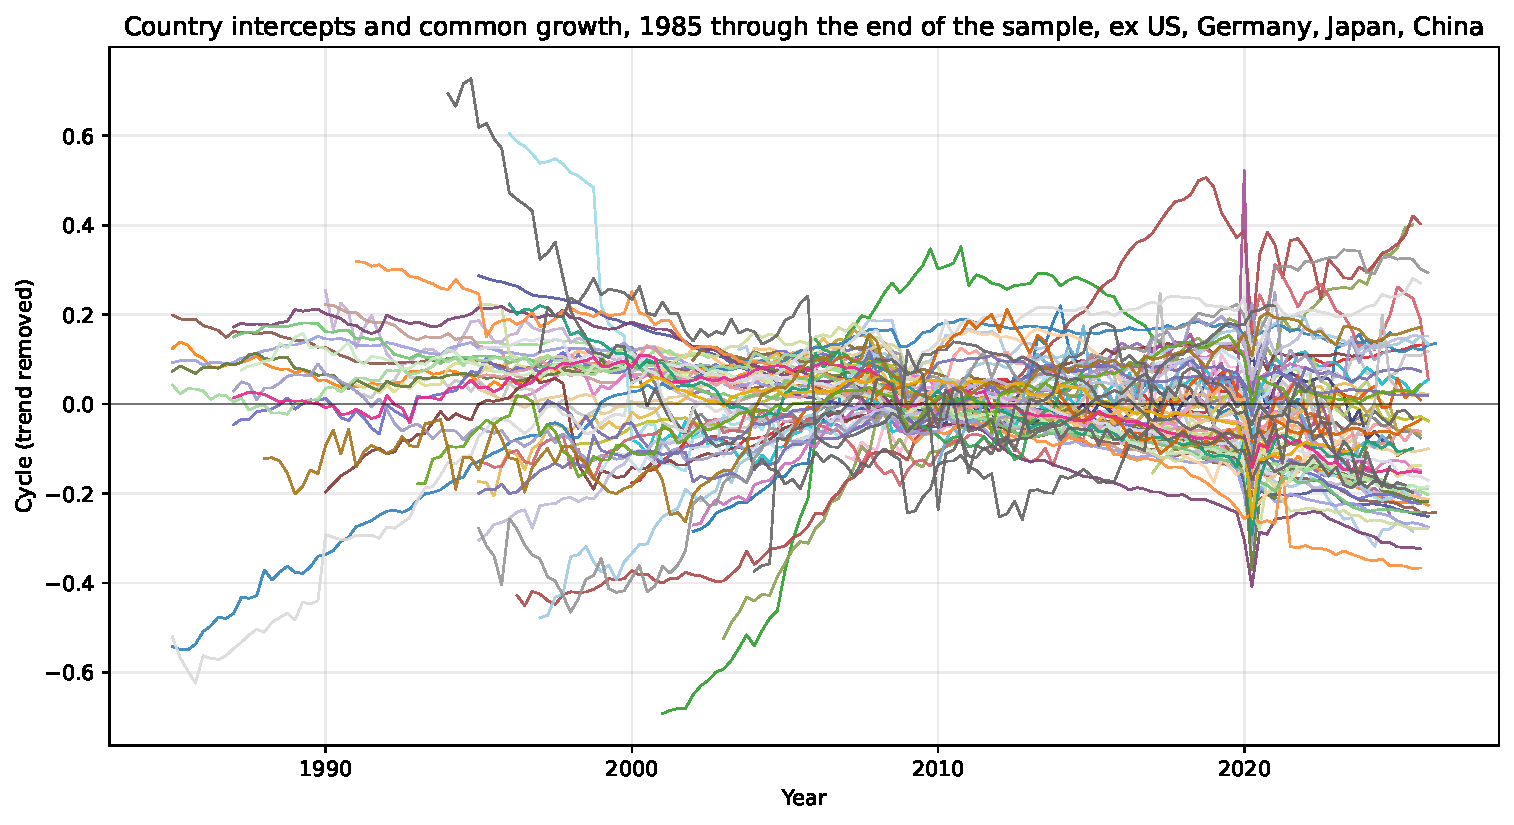
\includegraphics[width=0.75\textwidth]{figs/cycle_fe_1985.pdf}
\caption{Country cycles $z_{it}=y_{it}-a_i-gt$.}
\end{figure}
\end{document}
